\section{Path Generation Algorithm}\label{sec:pathgeneration}
The path generation algorithm creates a list of waypoints for the vessel to follow. The area that needs to be surveyed is used to generate the waypoints. The desired area is a bounded rectangle and is given as an input to the algorithm as four points, in \autoref{eq:pathgenxy}, that specify the limits of the area.
%
\begin{flalign} 
  \{x_1; y_1\},       \rule{15px}{0px} 
  \{x_2; y_2\},       \rule{15px}{0px}
  \{x_3; y_3\},       \rule{15px}{0px} 
  \{x_4; y_4\}.       \rule{15px}{0px} 
  \label{eq:pathgenxy}
\end{flalign}
%
\begin{where}
  \va{\{x_k; y_k\}}{is the coordinate of the corner of the bounded rectangle}{}
\end{where}

The path generation algorithm is confined to generate waypoints in an area that is a rectangle. Thus, the four input coordinates need to be verified to ensure the area is a rectangle. This is done by checking
\begin{flalign} 
  \sqrt{(x_1 - x_2)^2 + (y_1 - y_2)^2} &= \sqrt{(x_3 - x_4)^2 + (y_3 - y_4)^2} \ ,\\
  \sqrt{(x_1 - x_4)^2 + (y_1 - y_4)^2} &= \sqrt{(x_2 - x_3)^2 + (y_2 - y_3)^2} \ , \\
  \sin{\frac{y_1 - y_2}{x_1 - x_2}} - \sin{\frac{y_1 - y_4}{x_1 - x_4}}  &= \frac{\pi}{2} \ . 
  \label{eq:pathgen}
\end{flalign}
%
Now that the desired area is well defined, as a rectangle, the path generation algorithm is able to generate a list of waypoints for the ASV to follow.

The path is generated with straight lines and turns which the vessel shall follow. To determine the width between these lines, the dynamics of the vessel, the swath angle of the multibeam echosounder and the minimum depth of the area to survey were taken into consideration. The swath angle and minimum depth of the Port of Aalborg survey in \autoref{app:bathymetricMapPortOfAalborg} are used to calculate the width between straight lines, as described in \autoref{sec:designconsiderations},
%
\begin{flalign}
  w_\mathrm{beam} = 36\ \mathrm{m} \ .
\end{flalign}
\begin{where}
  \va{w_\mathrm{beam}}{is the minimum required beamwidth}{m}
\end{where}

The dynamics of the vessel are considered to ensure the vessel can perform smooth turns between straight lines. It is determined that the vessel is capable of using the turning radius 
%
\begin{flalign}
  R_\mathrm{turn} = \frac{1}{2} w_\mathrm{beam} = 18\ \mathrm{m} \ .
\end{flalign}
\begin{where}
  \va{R_\mathrm{turn}}{is the turning radius of the waypoints}{m}
\end{where}

The path generation algorithm first determines along which side of the rectangle to generate waypoints. This is done to ensure the vessel performs the least number of turns and is determined by calculating which side of the rectangle is larger. This is done by checking if
%
\begin{flalign}
	\sqrt{(x_1 - x_2)^2 + (y_1 - y_2)^2} \geq \sqrt{(x_1 - x_4)^2 + (y_1 - y_4)^2} \ .
\end{flalign}
%
Once the sailing direction is chosen, the first waypoint is generated using the starting point's coordinates and the direction of the straight lines. The starting point in the transversal direction is offset by $R_\mathrm{turn}$ so the multibeam starts surveying from the edges of the area.

The number of waypoints on both the straight lines and on the turns are generated using
%
\begin{flalign}
  d_\mathrm{wps} &= 50\ \mathrm{m} \ ,\\
  n_\mathrm{wps} &= 10 \ .
\end{flalign}
\begin{where}
  \va{d_\mathrm{wps}}{is the distance between waypoints on the straight line}{m}
  \va{n_\mathrm{wps}}{is the number of waypoints on each turn}{}
\end{where}

As the area to survey may vary, the waypoints are generated every $d_\mathrm{wps}$ to ensure the vessel converges faster if it diverges from the path. Thus, the vessel does not rely only on the waypoints that define the area. The path has a fixed turning radius, $R_\mathrm{turn}$, and therefore the number of waypoints is fixed to $n_\mathrm{wps}$.

In \autoref{fig:pathgen1} an example of the desired area to survey and the generated waypoints are shown. It can be seen that the vessel is offset by $R_\mathrm{turn}$ and the minimum area the multibeam sensor surveys is also shown.
%
\begin{figure}[H]
  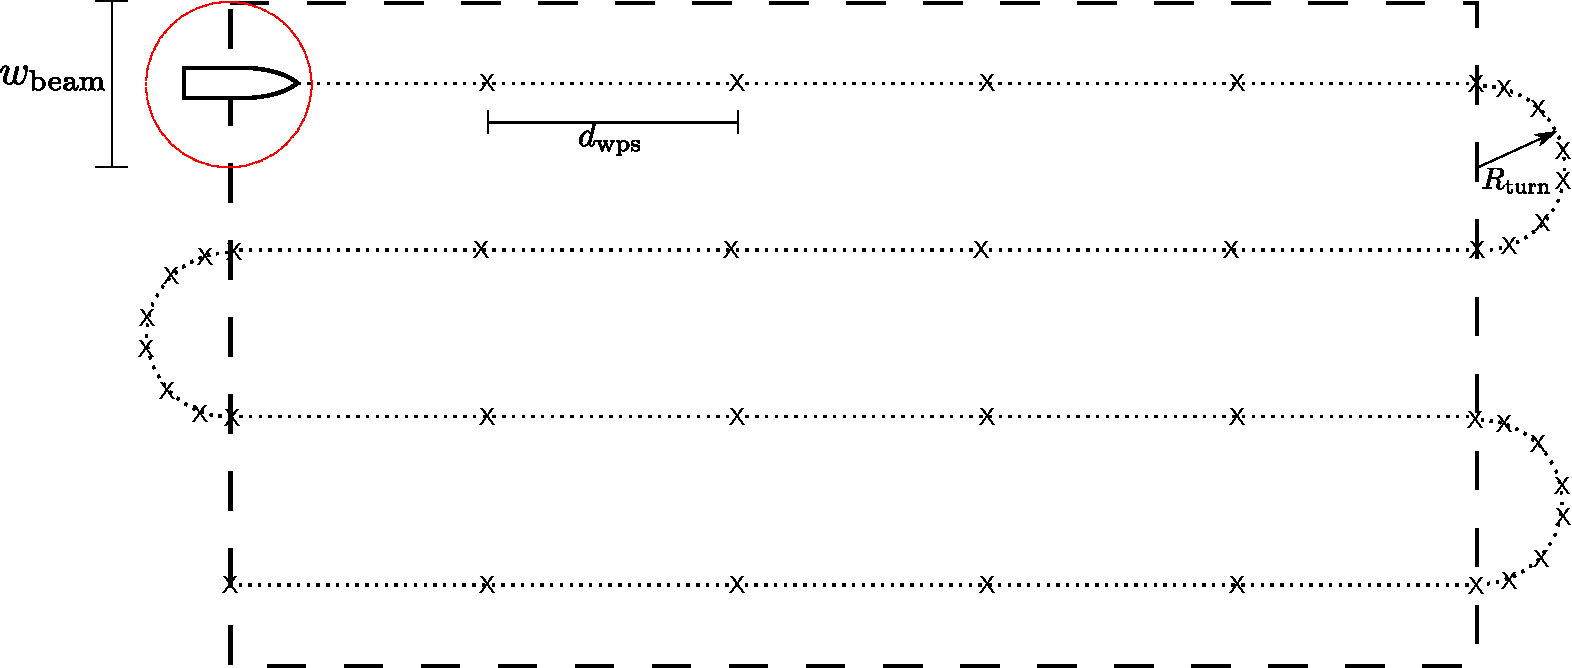
\includegraphics[width=1\textwidth]{figures/pathGen} 
  \caption{Area wanted to survey with waypoints.}
  \label{fig:pathgen1}
\end{figure}   


